\documentclass{sig-alternate}


\usepackage[latin1]{inputenc}
\usepackage{amssymb}
\setcounter{tocdepth}{3}
\usepackage{graphicx}
\usepackage{subfigure}

\usepackage{url}

\begin{document}

\title{Modeling browser-based distributed evolutionary computation systems} 

\numberofauthors{1} %  in this sample file, there are a *total*
% of EIGHT authors. SIX appear on the 'first-page' (for formatting
% reasons) and the remaining two appear in the \additionalauthors section.
%
\author{
% You can go ahead and credit any number of authors here,
% e.g. one 'row of three' or two rows (consisting of one row of three
% and a second row of one, two or three).
%
% The command \alignauthor (no curly braces needed) should
% precede each author name, affiliation/snail-mail address and
% e-mail address. Additionally, tag each line of
% affiliation/address with \affaddr, and tag the
% e-mail address with \email.
%
% 1st. author
\alignauthor
Som E. One\\
       \affaddr{Some Institute}\\
       \email{em@a.il}
}


\maketitle

\begin{abstract}
From the era of big science we are back to the "do it yourself", where
you do not have any money to buy clusters or subscribe to grids but
still have algorithms that crave many computing nodes and need them to
measure scalability. Fortunately, this coincides with the era of big
data, cloud computing, and browsers that include JavaScript virtual
machines. Those are the reasons why this paper will focus on two
different aspects of volunteer or freeriding computing: first, the
pragmatic: where to find those resources, which ones can be used, what
kind of support you have to give them; and then, the theoretical: how
evolutionary algorithms can be adapted to a environment in which nodes
come and go, have different computing capabilities and operate in
complete asynchrony of each other. We will examine the setup needed to
create a very simple distributed evolutionary algorithm using
JavaScript and then find a model of how users react to it by
collecting data from several experiments featuring different classical
benchmark functions. 
\end{abstract}

\keywords{Evolutionary computation, volunteer computing, distributed
  computing, node.js, javascript}

\section{Introduction}

The world has computational resources in spades. Most of them do not
belong to you or your lab. That does not mean you cannot use it. The
problem is how. 

Most theory in parallel computing has been devoted to predict and
optimize the performance in systems where the number of nodes, their
connections, and the time every one is devoting to the computation is
known in advance. However, even if Big Science is not really over and
it is slated to come back, the era of
Citizen Science already started a few years ago (with SETI@home \cite{david-seti:home} and then BOINC \cite{boinc_grid04}) and it
offers a vast amount of computational resources to attract, if only
you know how. But there is a challenge: knowing, or at least having a
ballpark, of how your algorithm is going to perform in this uncertain
environment, where none of the factors is known: neither the number of
nodes, through how they are connected, to how long are they going to
be focused on doing what you want them to. That is why some effort is
needed to first understand the dynamics of the decision to participate
in an experiment that requires you to click on a link and then stay
for a while looking at the screen (or just leave it there running).

Besides, since Amazon started selling EC2 several years ago, reliable
and scalable computing resources are also available for a low price
and on demand. Recently, Google has also refurbished its offering
lowering their prices. This means that the conjunction of free or
low-cost cloud computing engines, volunteer computing systems and and
untapped capability of desktop systems can be used for creating
massive, or at least potentially massive, distributed computing
experiments. These experiments can be easily created using open-source
repository sites like GitHub and deployed automatically to Platform as
a Service products such as Heroku or OpenShift. 

In general, any volunteer computing experiment will have to be made
``in the open''. The fact that somebody is giving you, basically for
free, computing resources, means that the scientist using them has to
give back. The baseline is releasing the source code used: all
volunteer computing platforms, from SETI@home on, have done it. The
opposite is probably the reason why many companies like PopularPower \cite{buyya2001compute}
have folded or others like CrowdProcess have decided to turn their
product to in-house computation: there must be a mutual relationship
of trust among the scientist and the person that is running his/her
code in the browser. As has been mentioned in the early stages of what
was then called {\em desktop grid computing}, \cite{gc:bausch}, in
fact CPU cycle selling might not make economic sense since there are
not so much demand for it and supply is quite high. However, while
potential supply is in fact huge, {\em actual} supply will depend on
the person holding it willing to actually allocate it to a particular
company selling it or a particular experiment needing it, not to
mention the fact that the experiment {\em actually} has to draw the
attention of the supplier. That is why trust is essential, and using
free software might not be enough: Openness
has to progress from open source code to open science: releasing all
data obtained in the experiment in a repository such as GitHub,
mentioned above, and even allowing real-time access to experiment data
to users.

Another possible reason of the failure of former companies to create a
for-profit desktop grid might be the lack of a way to predict what is
going to be that supply in a particular moment. It is impossible to
predict, in advance, to know how many persons  are going to visit a
particular website. Even if you pull all the resources you have and
they lie across continents and time zones, the number of cycles
apportioned to a particular experiment will depend not only on the
users lending their web real state to the experiments (which is
usually the case for cycle brokerage companies) but especially to
users going to a web site and spending some time on them. Even if it
is theoretically impossible to predict to a high precision what
happens, it is in practice possible to approximate the number of
visits in a site, at least in a particular one, using time series. But
in the short term and using a more general model, there is still need
to model the behavior of users so that more factors can be added to
the model other than the time series. This user behavior, of course,
presupposes that you are respecting their anonymity and privacy (not using
cookies, for instance) and that you are respecting the open approach
mentioned above. All computation can be done without the knowledge of
the user \cite{unwitting-ec}, but this would work against openness
that would, curiously enough, result in a huge decrease of the future
performance of any experiment you might want to perform. 

These are best practices that have been followed in the experiments in
this paper, that first presents the first versions of a platform for
distributed evolutionary algorithms using the browser and a free (as
in free beer) backend, and second, shows the result from an
statistical point of view in order to put the basis for a model of the
metacomputer obtained by joining all volunteers and the free backend
used for the experiment. This is not an exhaustive or complete
exploration of the possibilities of this kind of computation, but it
is enough to present the free software used to perform the experiments
and will allow us to describe, in general, the behavior of the users
as well as the performance achieved on the experiments done so far,
which should show some advantage over doing the same kind of
experiments locally using available resources. 

The rest of the paper is organized as follows: next we will present
the state of the art in volunteer computing and its modelization. We
will proceed to describe the experimental setup in Section
\ref{sec:exp}, some preliminary results in Section \ref{sec:res} and
finally we will present our conclusions in Section \ref{sec:conc}
along with future lines of work. 

\section{State of the art}
\label{sec:soa}

Using the web as a resource for distributed, or plainly user based,
evolutionary computation has a long history since JavaScript was
introduced as a browser-based language in 1997 and even before, when
other procedures, including Flash animations, VBScript, ActiveX or Java applets were
used. Java was pointed out in \cite{soares1998get} as a ``language for
internet'' and
\begin{quote}
Java can bring some important advantages... solves architectural
heterogeneity [...] easy to install and [...] built-in security
mechanisms
\end{quote}
The same paper by Soares et al. describes JET, a system that supports
the execution of parallel applications over the Internet. In fact the
same paper describes some other systems working at the same time,
except they cannot be used for science since they do not have a
comprehensive statistics support like JET. 

However, Java (and all the other technologies) is not universal in the
sense than an extra component, namely, the Java virtual machine, has
to be installed in the browser. JavaScript
\cite{flanagan2006javascript} was introduced in 1997 as a
browser-embedded language and has, since them, become a set of standards
\cite{ECMA-262} for the language, its components and future versions
that have been widely adopted by the industry and also by scientists,
who used them for creating a non-distributed evolutionary algorithm on
the browser as early as 1998 \cite{jj-ppsn98}. 

The potential for volunteer computing using browsers was realized
later on \cite{sarmenta-bayanihan} as well as the potential for
mischief of users with code in their hands
\cite{sarmenta-sabotagetolerance} however, these early efforts by
Sarmenta once again used Java and not JavaScript, making this effort
less universal. JavaScript can be used either for unwitting
\cite{unwitting-ec} or volunteer
\cite{langdon:2005:metas,gecco07:workshop:dcor} distributed
evolutionary computation and has been used ever since by several
authors, including more recent efforts \cite{Desell:2008:AHG:1389095.1389273,duda2013distributed,DBLP:journals/corr/abs-0801-1210} that even
used the client's GPU \cite{duda2013gpu}. Many other researchers have
used Java \cite{chong:1999:jDGPi} and others have gone away from the
server-based paradigm to embrace peer to peer systems
\cite{jin2006constructing,10.1109/ICICSE.2008.99}. These computing
platform avoid single points of failure (the server) but, since they
need a certain amount of infrastructure installed to start, the
threshold to join them is much lower. 

There have been relatively few efforts to analyze what is the
performance that can be obtained from these volunteer computing
effort. There was some effort initially to dodge the issue by making
the algorithm adaptive to the kind of resources allotted to it
\cite{milani2004online}, which is actually not such a big problem in
algorithms such as the evolutionary algorithm that can easily be
paralelized via population splitting or farming out evaluations to all
the nodes available. Lately, several approaches have focused on the
fault-tolerance of volunteer algorithms
\cite{gonzalez2010characterizing} which can, of course, be studied in
a more general distributed computing context
\cite{nogueras2015studying} or including it in a more general study of
performance of the evolutionary algorithm itself
\cite{DBLP:journals/gpem/LaredoBGVAGF14}. But the raw material of
volunteer computing, number of users and the time spent in the
computation in browser-based volunteer computing experiments, have only been studied in a limited way in
\cite{DBLP:journals/gpem/LaredoBGVAGF14} on the basis of a single
run. Studies using volunteer computing platforms such as SETI@home
\cite{javadi2009mining} found out that the Weibull, log-normal and Gamma distribution
modeled quite well the availability of resources in several clusters
of that framework; the shape of those distributions is a skewed bell
with more resources in the {\em low} areas than in the high areas:
there are many users that give a small amount of cycles, while there
are just a few that give many cycles. This is in concordance with the
results obtained in \cite{agajaj}.

As far as we know, this is the only experiment that uses computational
resources that are as dissimilar as smartphones and powerful laptops
or desktop computers in a research center. The methodology used to
gather resources and the algorithms used will be described next. 

\section{Methodology}
\label{sec:exp}

\begin{figure*}[h!tb]
  \centering
  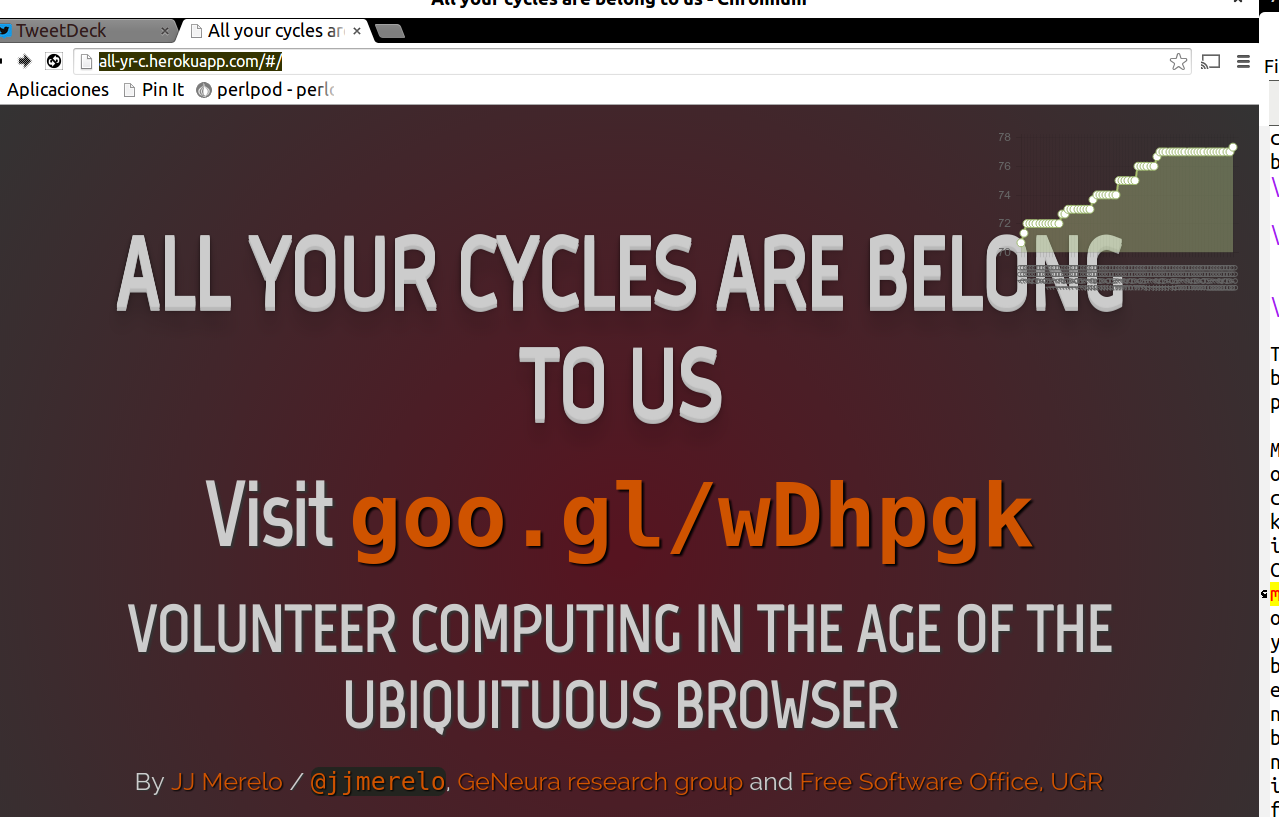
\includegraphics[trim=0cm 2cm 0cm 3cm, width=10cm]{img/screenshot.png}
  \label{fig:sshot}
  \caption{Screenshot of the talk that includes at the graph
    that shows the progression of the evolutionary
    algorithm at the top right corner}
\end{figure*}

In order to test the volunteer computing environment, a presentation
describing a low cost volunteer computing environment was
created. This presentation was actually delivered in several
conferences\footnote{Names withheld for the double blind review} and
it has the appearance shown in Figure \ref{fig:sshot}. During the
conference, it was revealed to the users that they were participating
in the experiment. The same procedure was used when trying to gather
users in social networks: a description of the container (the
presentation) and disclosure of its purpose. As it can be seen in the
image, the upper right corner shows the progress of the evolution. It
stops when the solution has been reached. 

Above the experiment, from the point of view of the user, has been
described. What it is actually running is an island model
\cite{muhlenbein1991parallel} in every browser that uses the server as
a {\em shuttle} to transfer individuals from one browser to another in
what can be eventually a fully connected topology. This deals with
several problems. The connection is stateless: islands connect to the
server to send and receive a single individual but there is no task
balancing: all islands start clicking on an URL and finish when they
browse off to the next page. Fault tolerance is implicit, in the sense
that no island has information that cannot be, or generated, somewhere
else, although if the server fails the experiment results might be
lost. All operation is asynchronous, with islands entering and leaving
the experiment all of their own. 

We will next explain its different parts from the point of
view of the architecture itself and the algorithm that it is actually
running. First we will describe the client code and next, in
subsection \ref{ss:server} the server architecture and where it is
hosted. 

\subsection{Volunteer distributed evolutionary computation in the browser}

\section{Results}
\label{sec:res}

\section{Conclusion}
\label{sec:conc}

In this paper we have presented our experience on using browser-based
computing applied
to the design of evolutionary algorithms.  

There are many issues involved in using these resources: from adapting current algorithms so that they match this environment \cite{agajaj} to check which EA configuration works the best in it, or creating a framework that can use it easily \cite{nodeo2014}. But the main challenge is that asking people to contribute resources implies that you are opening your science to society and you have to give something in return: you have to adopt a set of best practices that have come to be known as Open Science, because ``Give, and it shall be given unto you'', you will get as much back from society as you give to it opening your science and explaining it to the public. This, among other things, means that popularity will become directly performance of the metacomputer you create by attracting more users.


\bibliographystyle{abbrv}
\bibliography{geneura,volunteer,javascript,ror-js,GA-general}

\end{document}
